\documentclass[12pt, a4paper]{scrartcl}

%used packages
\usepackage[utf8]{inputenc}
\usepackage[ngerman]{babel}
\usepackage{xcolor}
\usepackage{graphicx}
\usepackage{hyperref}
\usepackage{makecell}
\usepackage{sectsty}
\usepackage{blindtext}

\usepackage{tabularx}
\usepackage{eurosym}
\usepackage{caption}
\usepackage{subcaption}


\usepackage{fancyhdr}
\pagestyle{fancy}
\renewcommand{\sectionmark}[1]{\markright{#1}}
\renewcommand{\footrulewidth}{0.4pt}
\fancyhead{}
\fancyhead[R]{\rightmark}
\fancyfoot{}
\fancyfoot[R]{\thepage}


%costum commads
\newcommand{\mailto}[1]{\href{mailto:#1}{\color{silver}{#1}}}
\newcommand{\NameMail}[2]{{{#1}}\\{\small\mailto{#2}}}
\newcommand{\mysubsection}[1]{\subsection*{#1}
	\addcontentsline{toc}{subsection}{#1}}

%color scheme
\definecolor{spaceCadet}{HTML}{2D3142}
\definecolor{independence}{HTML}{4F5F75}
\definecolor{silver}{HTML}{BFC0C0}
\definecolor{tumbleweed}{HTML}{D7A28A}
\definecolor{mandarin}{HTML}{EF8354}
\definecolor{sinopia}{HTML}{D12911}

%hyperref setup
\hypersetup{
	colorlinks,
	linkcolor=sinopia,
	citecolor={blue!50!black},
	urlcolor={sinopia!80!black}
}

%editig section and subsection style
\sectionfont{\color{spaceCadet}}
\subsectionfont{\color{independence}}
\subsubsectionfont{\color{tumbleweed}}

\begin{document}
	\begin{titlepage}
		\raggedleft
		
		\textcolor{mandarin}{\rule{1pt}{\textheight}} 
		\hspace{0.05\textwidth}
		\parbox[b]{0.85\textwidth}{
			
			{\Huge\bfseries \textcolor{spaceCadet}{SmartMirror}}\\[1\baselineskip]
			{\LARGE \bfseries \textcolor{independence}{Fakultät Informatik Mathematik}}\\[1\baselineskip]
			{\Large  \textcolor{independence}{OTH Regensburg}}\\[1\baselineskip]
			{\large \textcolor{independence}{Human Computer Interaction}}\\[2\baselineskip]
			
			
			
			
			{\LARGE\bfseries\textcolor{spaceCadet}{Projektbericht}}\\[0.2\baselineskip]
			{\Large\textcolor{independence}{Wintersemester 2020/2021}} \\[0.2\baselineskip]
			{\textcolor{independence}{\noindent 12. Februar 2021}} \\[3\baselineskip]
			
			\vspace{0.4\textheight}
			\begin{tabular}{ c c }
				\makecell[l]{\NameMail{Patrick Gruber}{patrick.gruber@st.oth-regensburg.de}}
				& \makecell[l]{\NameMail{Tobias Gubo}{tobias1.gubo@st.oth-regensburg.de}}\\
				\makecell[l]{\NameMail{Michael Lazik}{michael1.lazik@st.oth-regensburg.de}} 
				& \makecell[l]{\NameMail{Marcus Müller}{marcus.mueller@st.oth-regensburg.de}}
			\end{tabular}\\ [2\baselineskip]
		}
		
	\end{titlepage}
	
	\tableofcontents
	\thispagestyle{empty}
	\pagebreak
	\setcounter{page}{1}
	
	\section{Planen des menschzentrierten Gestaltungsprozesses}
	\begin{quote}
		{Nur wer sein Ziel kennt, findet den Weg.} - Laozi
	\end{quote}
	Wie jedes gute Projekt beginnt man mit der grundlegenden Planung und Strukturierung 
	\subsection{Festlegen der Resourcen}
	Der erste und elemetarste Schritt war es sich zu überlegen, wie ein Produkt wie der SmartMirror überhaupt realisiert werden kann. Dafür haben wir uns im Internet auf die Suche gemacht und sind dort an mehreren Stellen auf DIY-Projekte gestoßen, die eine ähnliche Idee umgesetzt haben. Die fundamentalen Bestandteile waren jedoch oft sehr vergleichbar. Man benötigt einen Einwegspiegel, der das Licht von einer Seite durchlässt und von der anderen Seite verspiegelt ist. Mit einem LED-Display hinter der Spiegelscheibe lässt sich so eine Anzeigefläche erschaffen, die für den Betrachter nur sichtbar ist, wenn sie beleuchtet ist. Die Art und Weiße, wie das Display angesprochen wird ist wieder eine freiere Entscheidung. Wir haben uns dafür entschieden einen RaspberryPi 3b zu verwenden. Dies hat mehrere Gründe, die im Laufe des Berichts noch genauer beleuchtet werden.Montiert wird das Spiegeldisplay in einem Rahmen aus Holz, um ein einheitliches Erscheinungsbild zu kreieren. Als letztes wichtiges Element ist noch der LeapMotion-Controller zu nennen, der eine einfache Möglichkeit bildet um die Gestik des Nutzers zu erkennen, um somit die Interaktion zwischen Mensch und Maschine zu ermöglichen.
	
	\subsubsection*{Grobe Kostenaufstellung}
	\begin{tabularx}{0.95\textwidth}{|X|l|r|}
		\hline
		\textcolor{tumbleweed}{\underline{\textbf{Name}}} & \textcolor{tumbleweed}{\underline{\textbf{Zulieferer}}} & \textcolor{tumbleweed}{\underline{\textbf{Preis}}}\\
		\hline
		Spiegelglas 70x100cm & GlasStar&ca. 125\euro\\
		\hline
		Display 17" mit Controller & Amazon & ca. 160\euro\\
		\hline
		LeapMotion Controller & AdaFruit & ca. 100\euro \\
		\hline
		Holzrahmen 70x100cm & Amazon & ca. 50\euro\\
		\hline
		Raspberry Pi & Amazon & ca. 40\euro\\
		\hline
		Kabel und Verbidungen & Amazin & ca. 50\euro\\
		\hline
		\textcolor{tumbleweed}{\textbf{Gesamt}}& & \textbf{ca. 525\euro}\\
		\hline
	\end{tabularx}
	
	\subsection*{Aufgabenaufteilung}
	\begin{tabularx}{0.95\textwidth}{|l|X|}
		\hline
		Patrick Gruber & Erstellen der Kostenaufstellung\\
		\hline
		Tobias Gubo & \\
		\hline
		Michael Lazik & \\
		\hline
		Marcus Müller & \\
		\hline
	\end{tabularx}
	
	\newpage
	
	\section{Verstehen und Festlegen des Nutzungskontexts}
	Nachdem die Ressourcen festgelegt worden sind, musste der Nutzungskontext definiert, verstanden und festgelegt werden. Hierbei wurde überlegt, wer die Benutzer sind und wie die Benutzer mit dem Smart Mirror interagieren werden.
	\subsection{Beschreibung des Nutzungskontexts}
	Unsere Primären (Direkten) Benutzer sind die Probanden, die unser Smart Mirror testen und Fazite daraus ziehen.\\
	Die Sekundären (Indirekten) Benutzer sind die Mitglieder des Projektteams, die aus den Fazite den Smart Mirror weiter entwickeln.\\
	Mit dem Smart Mirror sollen den Benutzern innerhalb kürzester Zeit die wichtigsten Informationen am Spiegel gezeigt werden.\\
	Dabei sollen dem Benutzer gezeigt werden:
	\begin{itemize}
		\setlength\itemsep{-0.5em}
		\item Uhrzeit
		\item Wetter (Uhrzeitbedingt)
		\item RSS-Feed
	\end{itemize}
	Zudem kann der Benutzer seine individuellen Informationen anzeigen lassen. In unserem Projekt sind das:
	\begin{itemize}
		\setlength\itemsep{-0.5em}
		\item Termine
		\item  ToDo-Liste
		\item Fahrzeiten ÖPNV
		\item Verkehrslage
		\item Speißeplan
	\end{itemize}
	Für den Smart Mirror benötigt der Nutzer keine Ausrüstung. Sie müssen nur wissen, wie man mit dem Smart Mirror interagiert und wie man durch den Pageflow die Seiten wechselt. Der Smart Mirror kann an jeden von den Benutzern beliebig ausgewählten Ort stehen. Das Projektteam hat sich jedoch auf das Schlafzimmer als Örtlichkeit für den Smart Mirror festgelegt.\\
	
	Damit der Nutzungskontext aus Sicht der primären Benutzer verstanden ist, wurden Interviews mit den Probanden geführt.
	Dabei wurden vor allem zu Beginn möglichst offene, neutrale und allgemeine Fragen gestellt, also das "Warum?", die dann immer mehr in die Materie des Smart Mirrors gingen, also das "Wie?". Hier konnten die Probanden aus ihre Vorstellung eines Smart Mirrors offenbaren und das Projektteam konnte anhand dieser Informationen die Nutzungsanforderungen festlegen. 
	

	
	
	\subsection*{Aufgabenaufteilung}
	\begin{tabularx}{0.95\textwidth}{|l|X|}
		\hline
		Patrick Gruber & \\
		\hline
		Tobias Gubo & \\
		\hline
		Michael Lazik & \\
		\hline
		Marcus Müller & \\
		\hline
	\end{tabularx}
	
	\newpage
	
	\section{Erarbeitung von Gestaltungslösungen zur Erfüllung des Nutzungskontexts}
	\subsection{Erstellen der Interaktionsspezifikation}
	Anhand der zuvor, durch Umfragen und Formulare erlangten Informationen über das potentielle Nutzungsverhaltens der User, wurden nun die möglichen Varianten der Interaktion mit dem Spiegel validiert.\\
	Dabei standen Folgende Optionen zur Verfügung:
	\begin{itemize}
		\setlength\itemsep{-0.5em}
		\item Toucheingabe
		\item Sprachsteuerung
		\item Gestensteuerung
	\end{itemize}
	Hierbei stellte sich heraus, dass die Sprachsteuerung oftmals von den Nutzern als negativ empfunden wurde, da hier das Gefühl entsteht, dass der Spiegel alles mithört was in der nähe davon gesprochen wird. Die Toucheingabe wurde ausgeschlossen, da hier einfach das Problem besteht, dass der Spiegel durch die Fingerabdrücke verschmutzt wird, sodass häufiges reinigen notwendig wäre.\\
	Letztendlich fiel die Wahl nun auf die Gestensteuerung, da hier die Umfragen aufzeigen, dass Gesten für viele Nutzer eine intuitive Möglichkeit darstellt, einen Spiegel zu bedienen.\\
	Daraufhin wurde noch validiert welche konkreten Gesten für den Nutzer am einfachsten zu benutzen waren. Diese Entscheidung geht Hand in Hand mit Punkt “4.2 Erstellen der Informationsarchitektur” da das Layout der Informationen eine maßgebliche Rolle für die Art wie darauf Navigiert werden muss, spielt.\\
	Dabei wurde das folgende Konzept herausgearbeitet:
	\begin{figure}[h!] 
		\centering
		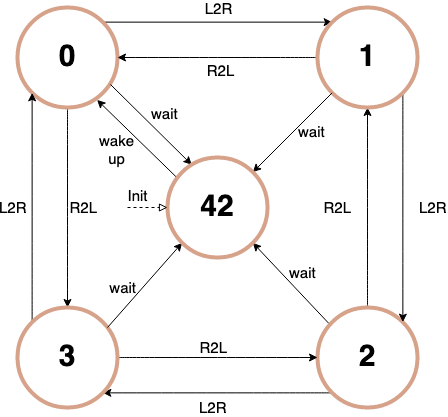
\includegraphics[width=0.4\textwidth]{img/Zustandsdiagramm.png}
		\captionsetup{labelformat=empty}
		\caption{Zustandsdiagramm des Systems}
	\end{figure}\\
	Auf diesem Bild ist zu sehen wie die 5 unterschiedlichen Seiten des Spiegels mittels den Gesten swipe Links nach Rechts oder swipe Rechts nach Links erreicht werden können.
	Diese beiden Gesten stellten für die grundsätzliche Bedienung die schönste Möglichkeit dar, den Spiegel zu bedienen. Zusätzlich können die Bewegungen swipe Hoch und swipe Runter für erweiterte Funktionalitäten wie Bildschirmhelligkeit oder Ähnliches genutzt werden.
	
	\subsection{Erstellen der Informationsarchitektur}
	Begonnen wurde die gestaltung der Informationsarchitektur mittels eines \href{https://trello.com/b/hdf8bWp2/sippin-on-my-lean-ux}{Trello-Boards}. Dabei wurden erst auf basis von Nutzer Feedback eine Sammlung an intressanten Features erstellt. Daraufhin wurde mittels \href{https://www.optimalworkshop.com/optimalsort/}{Optimal Workshop} und Card Sorting analysiert wie Nutzer Informationen und Features gruppieren würden. Das gab ein klares Bild über die Struktur der Informationen am Spiegel.
	\begin{figure}[h!]
		\centering
		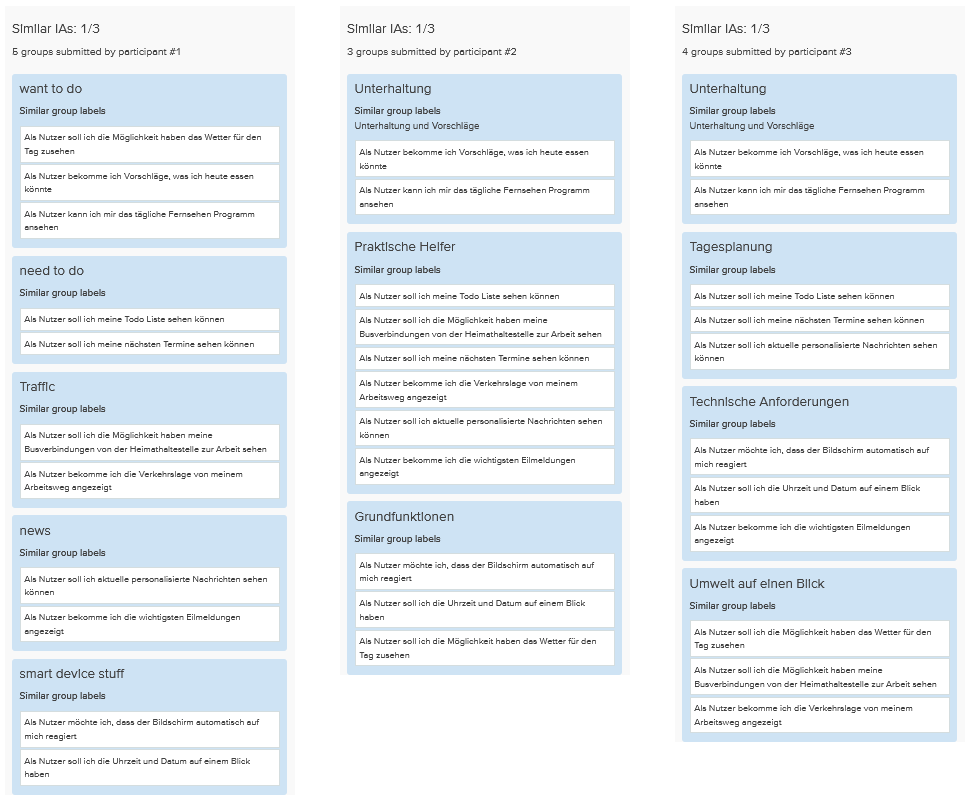
\includegraphics[width=\textwidth]{img/IA.png}
		\captionsetup{labelformat=empty}
		\caption{Informationarchitecture}
	\end{figure}
	\newpage
	Nachdem die Gruppen festgelegt wurden, zeichnete sich ein klares Bild ab, welche Features wie am Spiegel angezeigt werden solle:
	\begin{itemize}
		\item HomeScreen
		\begin{itemize}
			\item Uhrzeit
			\item Datum
		\end{itemize}
	\item Termine \& ToDo
	\begin{itemize}
		\item Termine für heute
		\item ToDo-Liste für heute
	\end{itemize}
	\item  ÖPNV
	\begin{itemize}
		\item Die Abfahrtszeiten vom aktuellen Standort zu einem festlegbaren Ort
	\end{itemize}
	\item  Verkehrslage
	\begin{itemize}
		\item Der aktuelle Weg zur Arbeit samt Stauinformation
	\end{itemize}
	\item Speißeplan
	\begin{itemize}
		\item Die Gerichte des heutige Tages
	\end{itemize}
	\end{itemize}
	
	
	\subsection{Spezifikation des UI}
	Die Entwicklung der UI begann mit Paper Prototyping. Hierbei wurden die ersten ersten Entwürfe auf basis der im vorherigen Schritt erstellten Informationsarchitektur erstellt.
	\begin{figure}[h!]
		\centering
		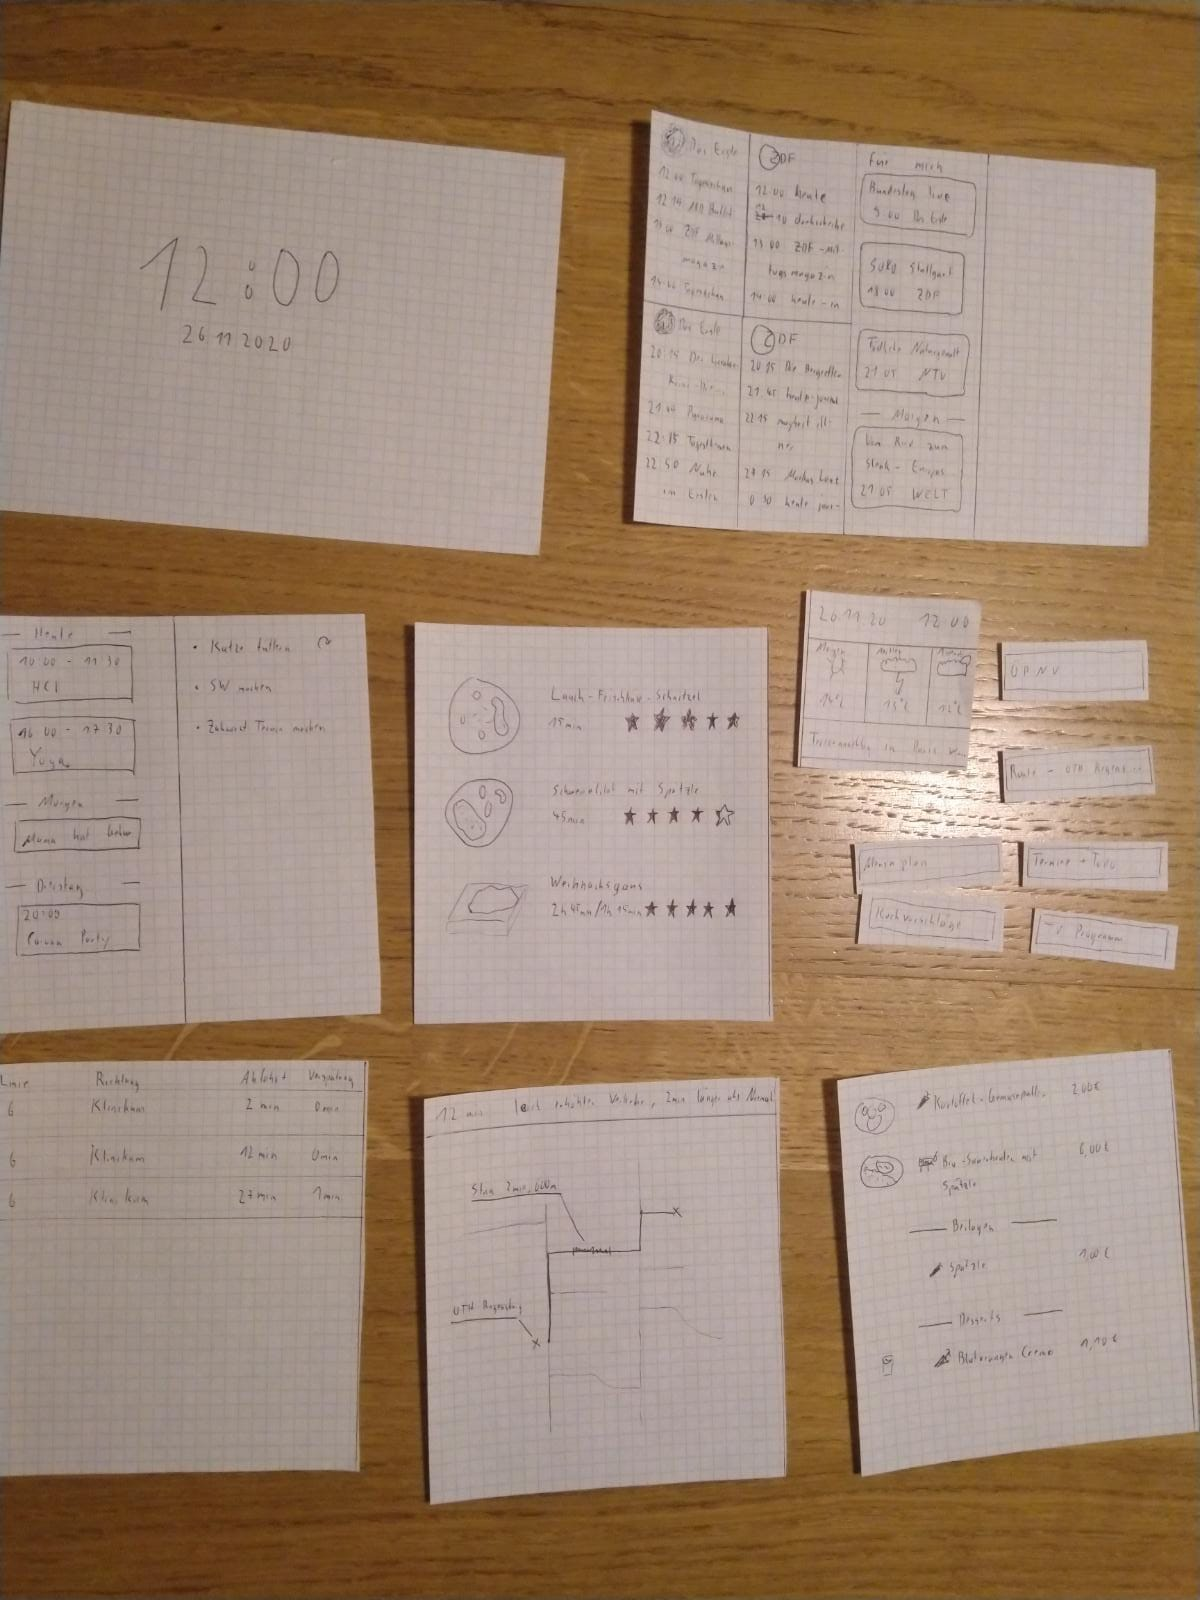
\includegraphics[width = 0.3\textwidth]{img/paperSketching.jpg}
		\captionsetup{labelformat=empty}
		\caption{Paper sketching}
	\end{figure}\\
	Danach ging es weiter mit dem Design der unterschiedlichen Seiten mittels Powerpoint. Hier wurden konkrete Designs mit den verschiedensten UI Elementen ausgearbeitet.
	
	\begin{figure}[h!]
		\begin{subfigure}{0.5\textwidth}
			\centering
			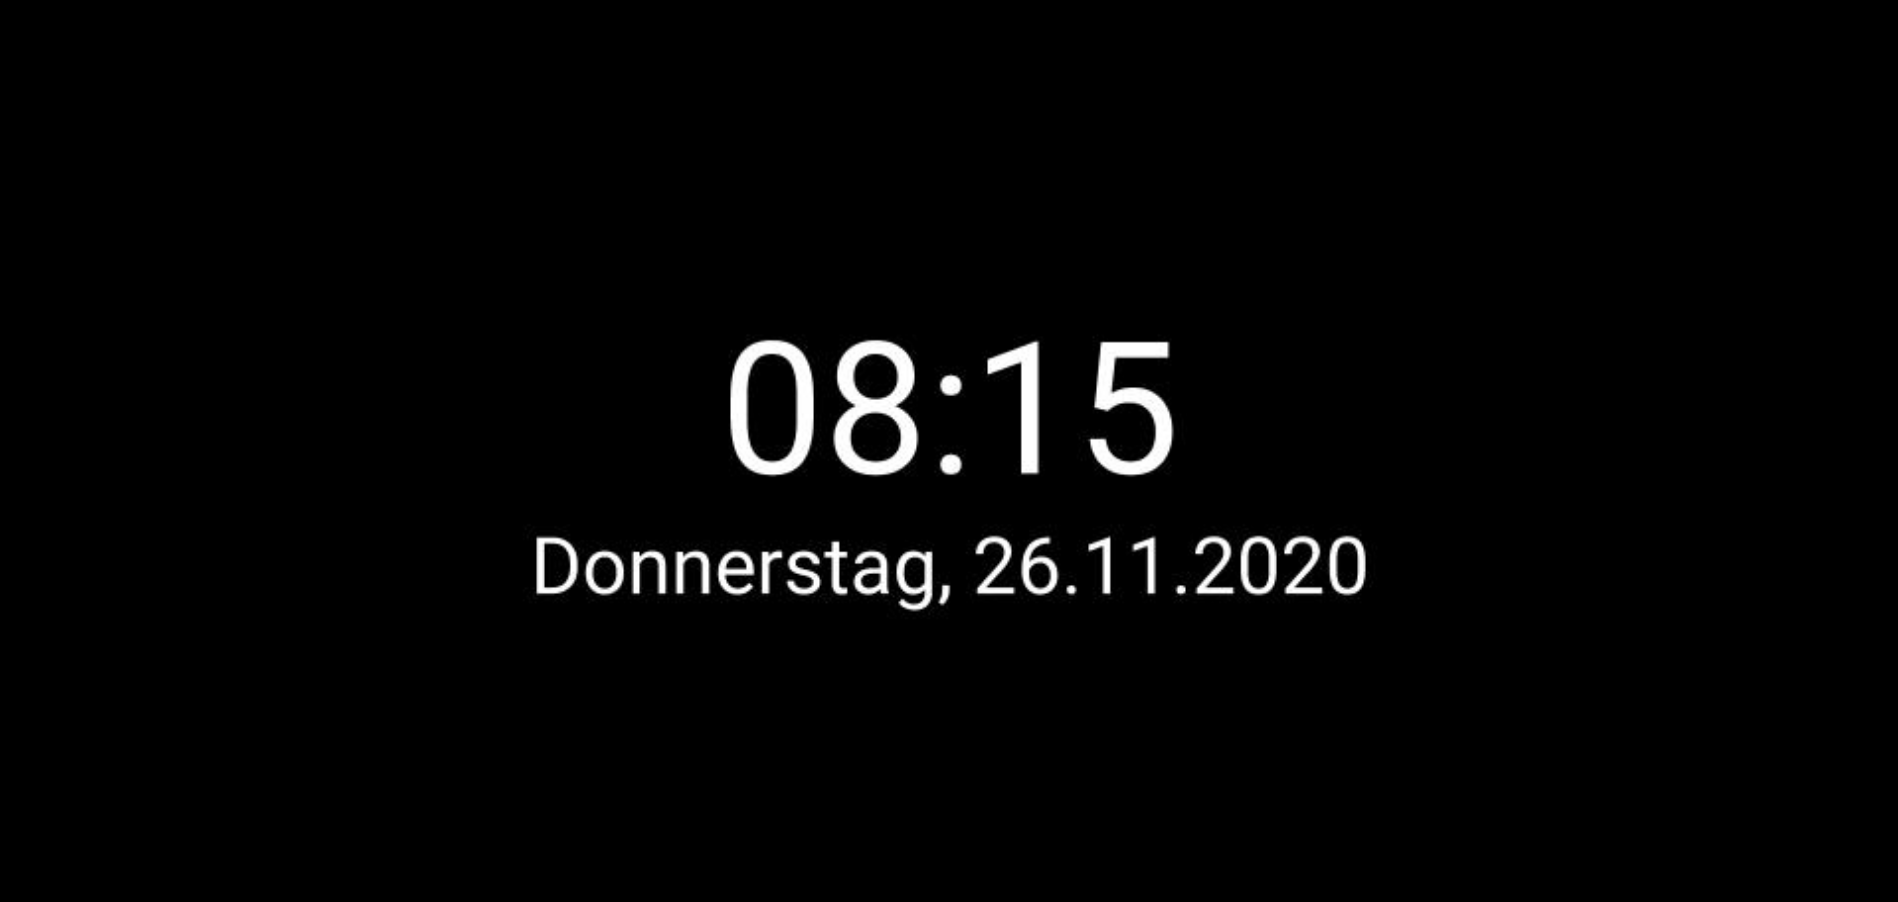
\includegraphics[width = 0.8\linewidth]{img/standby.png}
		\end{subfigure}
	\begin{subfigure}{0.5\textwidth}
	\centering
	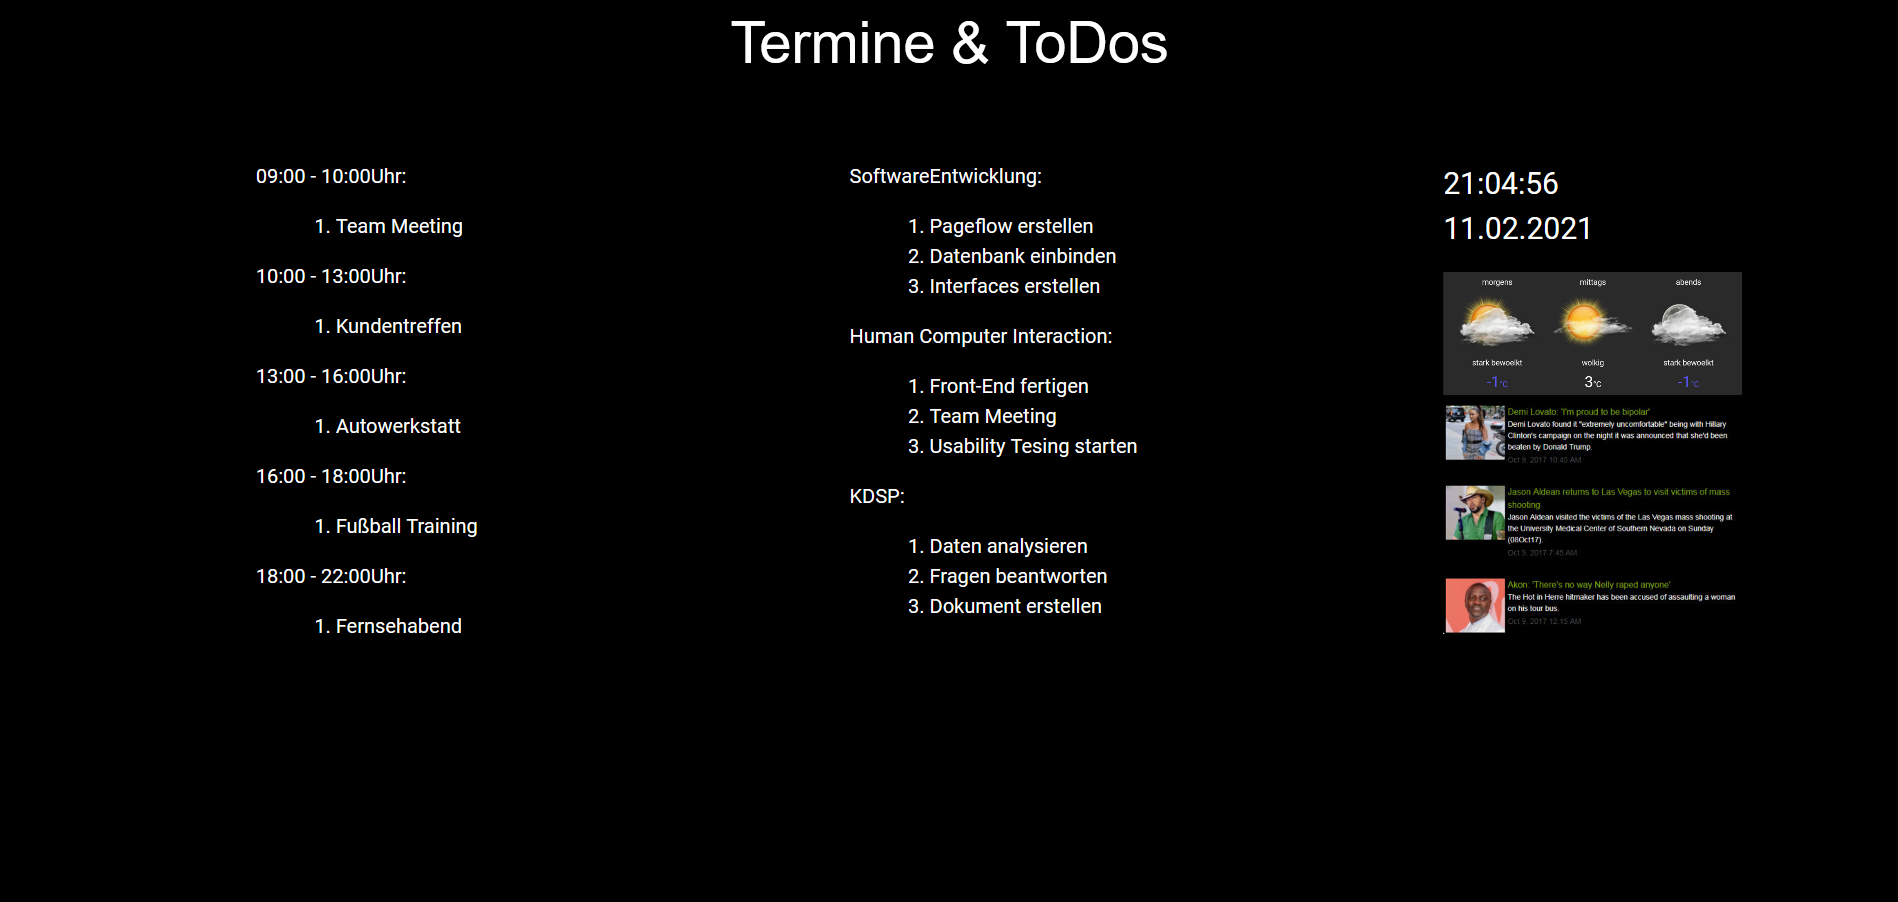
\includegraphics[width = 0.8\linewidth]{img/TermineToDo.png}
	\end{subfigure}
	\end{figure}	\begin{figure}[h!]
	\begin{subfigure}{0.5\textwidth}
		\centering
		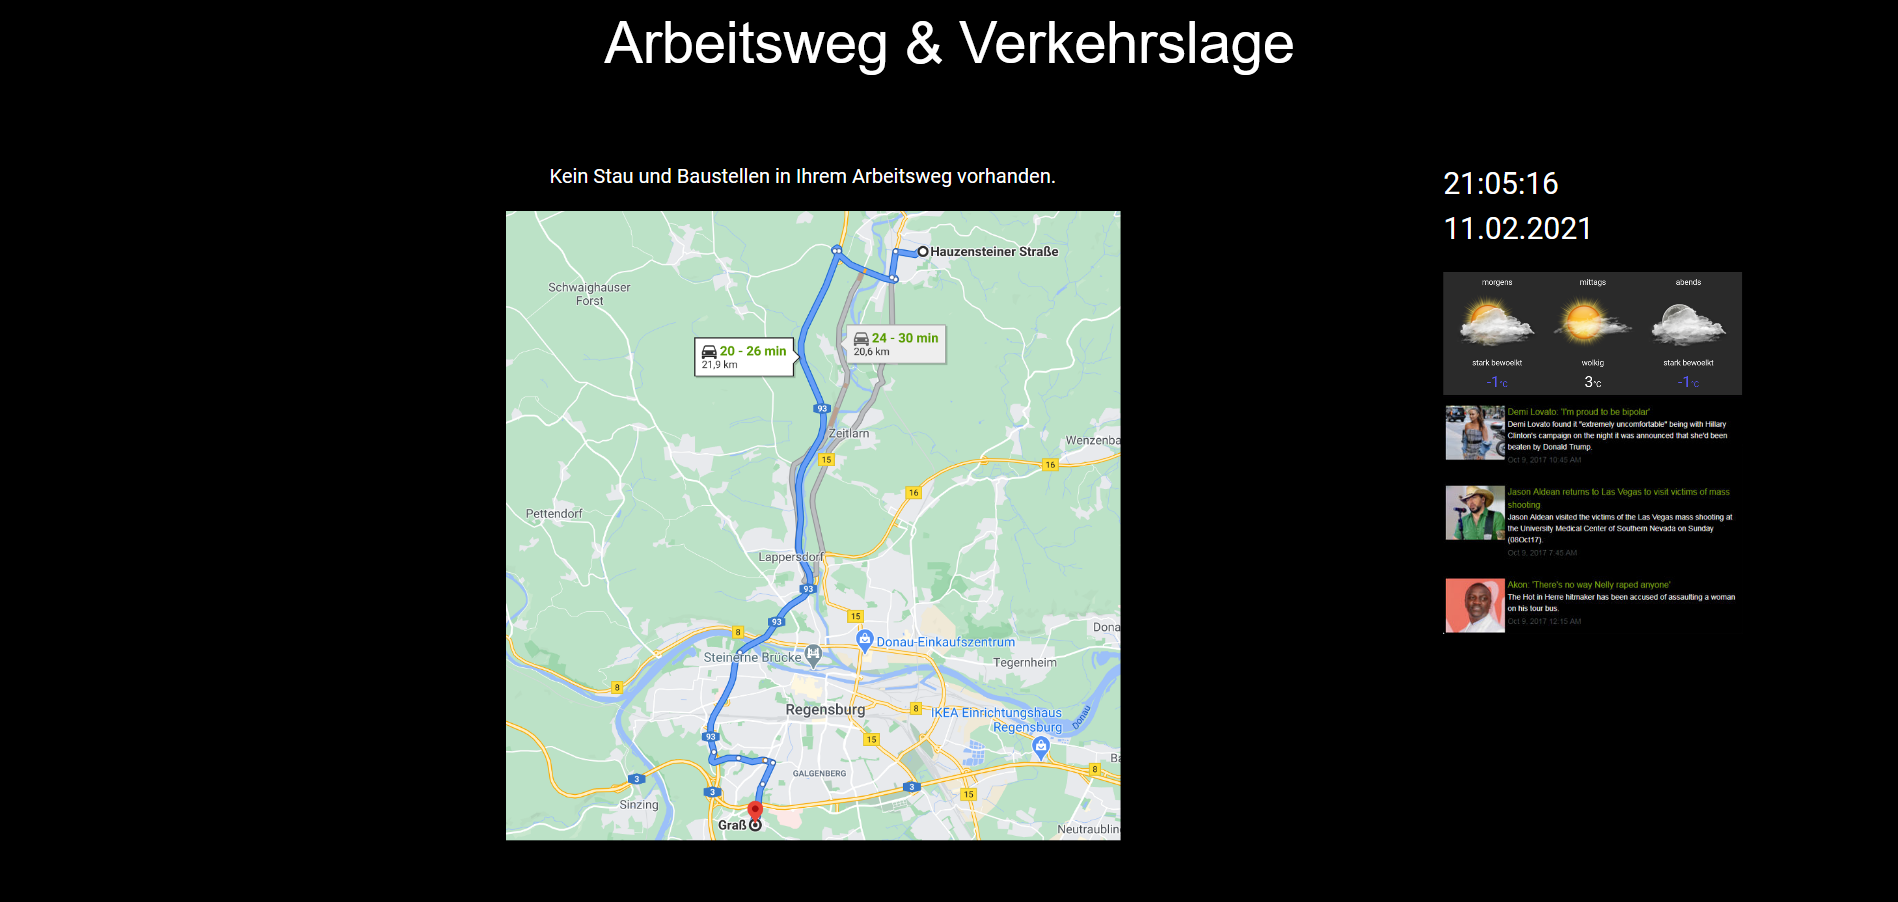
\includegraphics[width = 0.8\linewidth]{img/Arbeitsweg.png}
	\end{subfigure}
	\begin{subfigure}{0.5\textwidth}
		\centering
		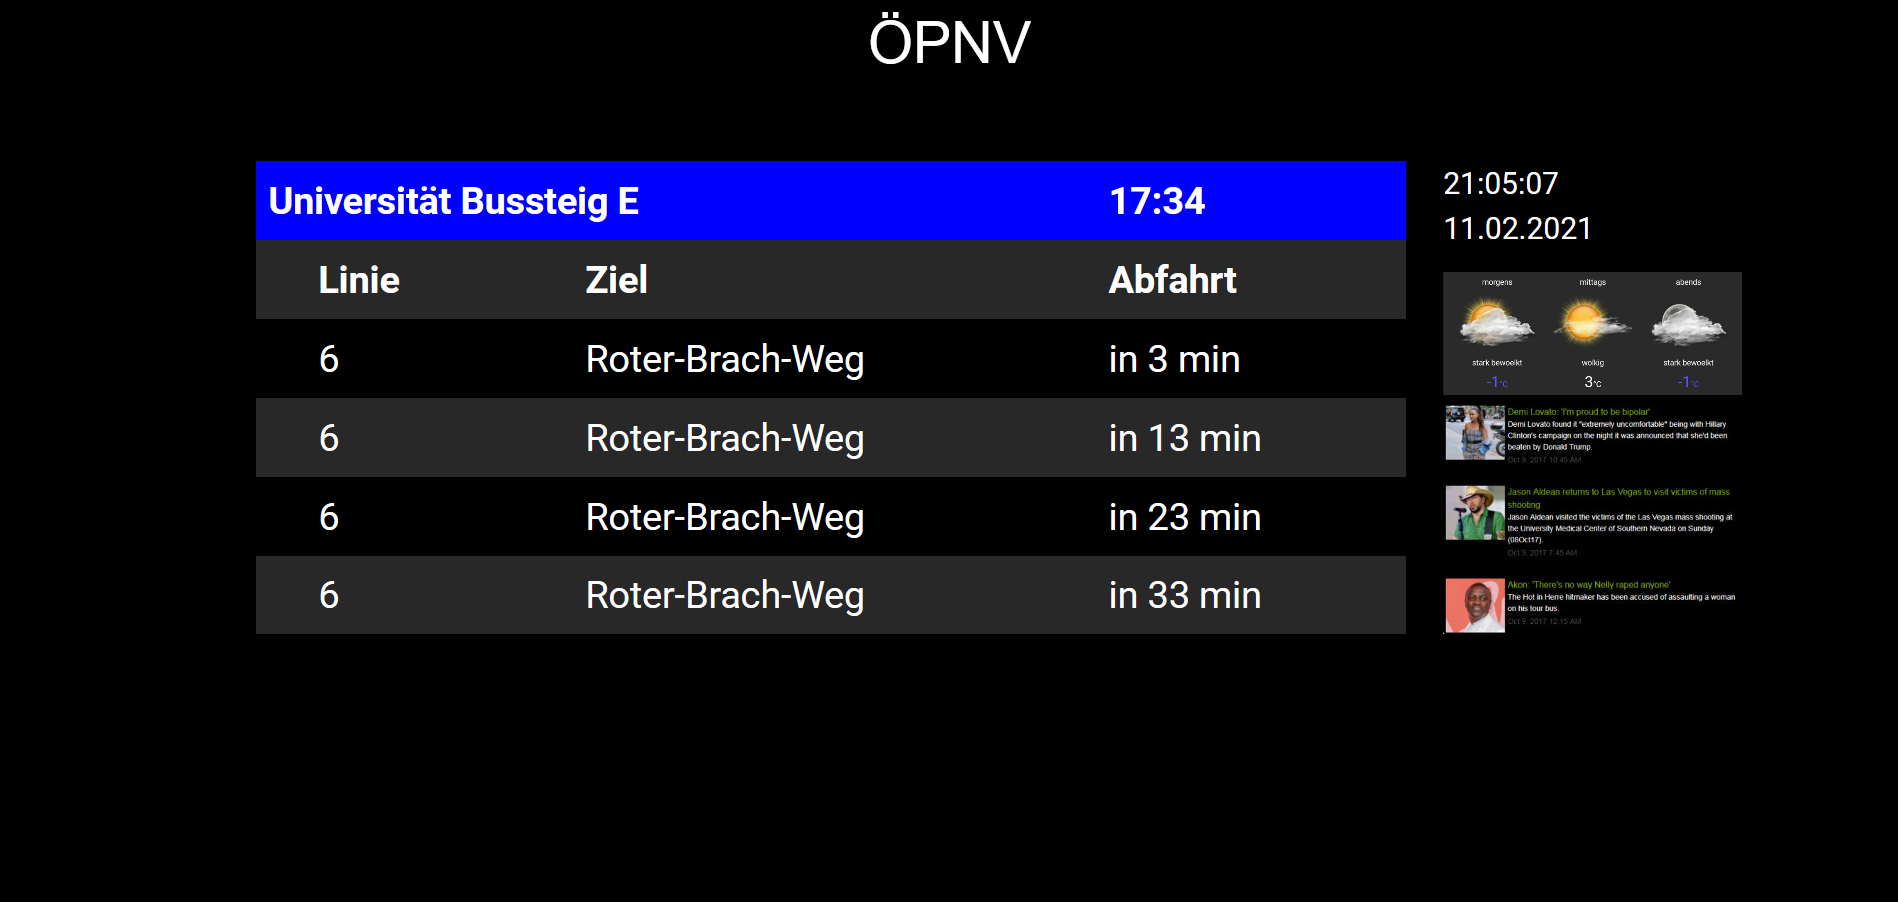
\includegraphics[width = 0.8\linewidth]{img/bus.png}
	\end{subfigure}
	\end{figure}	
	\begin{figure}[h!]
		\centering
		\includegraphics[width = 0.4\linewidth]{img/mensa.png}
	\end{figure}

	\subsection{Prototyping}
	Der Prototyp wurde mittels dem Frontend Framework vue.js und node.js als Backend entwickelt. Dabei wurden die einzelnen Seiten auf basis von den Powerpoint Designs in html Nachprogrammiert. Zur Steuerung des Spiegels wurde ein Leap Motion Sensor mittels des bereitgestellten JS SDKs in den node Server integriert. Darin wurde Gestenerkennung implementiert. Die erkannten gesten werden nun mittels Web Sockets an das vue.js Frontend gesendet. Hier wurden die Gesten nun zur Navigation des UIs verwendet.\\
	Aus Usability zwecken wurden zwei Varianten des Gestenerkennungs-Algorithmuses erstellt. Eine Version die die Gesten nach einer bestimmten Distanz auslöst (also mehrfach swipe mit einer Handbewegung möglich) und eine die bei einer Bewegung nur eine Geste erkennt. Nach User Testing stellte sich heraus, dass die zweite Variante deutlich intuitiver für den User ist, da diese immer versuchen, wie am Smartphone, durchgängige Wischgesten zu tätigen.\\
	Am Schluss wurde ein Konzept zur Durchführung von Usability Tests erstellt. Das erstellte Dokument enthält eine kurze Vorstellung des Projektes, Hinweise zum Usability Testing und Aufgaben, die der Teilnehmer am Spiegel durchführen soll. Die Aufgaben behandeln das Navigieren zwischen den Seiten und das Herauslesen von Informationen. Nach Durchführung des Tests sollen in einem offenen Gespräch zusätzliche Informationen gewonnen werden.
	
	
	\subsection{UI Gestaltungsrichtlinien}
	Um für ein vereinheitlichtes Design zu sorgen, wurde immer die gleiche Schriftart und die gleiche Hintergrundfarbe verwendet. Um Inkonsistenzen zu vermeiden, wurden Komponenten, die auf mehreren Seiten auf die gleiche Art und Weise dargestellt werden, als Fragment in die Seiten eingebunden. Das wären unter anderem diese Komponenten:
	\begin{itemize}
		\setlength{\itemsep}{-0.5em}
		\item Uhrzeit
		\item Wetter
		\item RSS-Feed
	\end{itemize}
	
	\subsection*{Aufgabenaufteilung}
	\begin{tabularx}{0.95\textwidth}{|l|X|}
		\hline
		Patrick Gruber & 
		\begin{itemize}
			\setlength{\itemsep}{-0.5em}
			\item  Validierung der Interaktionsmöglichkeiten
			\item  Entwurf der Navigations zwischen den Seiten
			\item Erstellen des Trello-Boards
			\item Durchführen des Card-Sortings
			\item Paper Prototyping
			\item Implementierung der Gestenerkennung
			\item Erstellung eines Konzepts zur Durchführung von Usability Tests am Prototypen
		\end{itemize}\\
		\hline
		Tobias Gubo & \begin{itemize}
			\setlength{\itemsep}{-0.5em}
			\item  Validierung der Interaktionsmöglichkeiten
			\item  Entwurf der Navigations zwischen den Seiten
			\item Erstellen des Trello-Boards
			\item Durchführen des Card-Sortings
			\item Paper Prototyping
			\item Prototyping Setup vo vue.JS und node.JS einrichten
			\item Implemetierung der Socket Kommunikation
			\item Implemetierung der Gestenerkennung
			\item Erstellung eines Konzepts zur Durchführung von Usability Tests am Prototypen
		\end{itemize} \\
		\hline
		Michael Lazik &  \begin{itemize}
			\setlength{\itemsep}{-0.5em}
			\item  Validierung der Interaktionsmöglichkeiten
			\item  Entwurf der Navigations zwischen den Seiten
			\item Erstellen des Trello-Boards
			\item Durchführen des Card-Sortings
			\item Paper Prototyping
			\item Implementierung der Spiegel UI mittels vue.JS
			\item Erstellung eines Konzepts zur Durchführung von Usability Tests am Prototypen
		\end{itemize}\\
		\hline
		Marcus Müller &  \begin{itemize}
			\setlength{\itemsep}{-0.5em}
			\item  Validierung der Interaktionsmöglichkeiten
			\item  Entwurf der Navigations zwischen den Seiten
			\item Erstellen des Trello-Boards
			\item Durchführen des Card-Sortings
			\item Paper Prototyping
			\item Erstellung eines Konzepts zur Durchführung von Usability Tests am Prototypen
		\end{itemize}\\
		\hline
	\end{tabularx}
	
	\newpage
	
	\section{Aufbau Software System}
	\subsection{System}
	\subsection{Frontend}
	\subsection{Backend}
	
	\subsection*{Aufgabenaufteilung}
	\begin{tabularx}{0.95\textwidth}{|l|X|}
		\hline
		Patrick Gruber & \\
		\hline
		Tobias Gubo & \\
		\hline
		Michael Lazik & \\
		\hline
		Marcus Müller & \\
		\hline
	\end{tabularx}
	
	\newpage
	
	\section{Evaluierung der Gestaltungslösung anhand der Nutzungsanforderung}
	\blindtext[2]
	\subsection{Entwicklungsbegleitende Usability-Tests}
	\blindtext[1]
	\subsection{QuantitativeEvaluierungen}
	
	
	\subsection*{Aufgabenaufteilung}
	\begin{tabularx}{0.95\textwidth}{|l|X|}
		\hline
		Patrick Gruber & \\
		\hline
		Tobias Gubo & \\
		\hline
		Michael Lazik & \\
		\hline
		Marcus Müller & \\
		\hline
	\end{tabularx}
	
	
	
\end{document}